\section{Exemplary Maps}
\label{sect:exemplary-maps}

In this section, we showcase a range of maps produced by our framework.
\Cref{fig:exemplary-maps-dynamics} shows how such a map evolves over time as the underlying cluster graph changes.
\Crefrange{fig:exemplary-maps-small}{fig:exemplary-maps-large} show representative maps for different numbers of regions $n \in \{10,20,30\}$.

\newcommand{\bigdrawing}[1]{\setlength\fboxsep{0pt}\colorbox{gray!10}{\makebox(190,190){\includegraphics[width=190pt,height=190pt,keepaspectratio]{#1}}}}
\newcommand{\smalldrawing}[1]{\setlength\fboxsep{0pt}\colorbox{gray!10}{\makebox(120,111){\includegraphics[width=120pt,height=111pt,keepaspectratio]{#1}}}}

\begin{figure}[H]
\centering
\begin{tabular}{lc}
\begin{minipage}{0.62\textwidth}
\subfigure[]{\smalldrawing{Resources/Evaluation-Example-Dynamics-AE097F3A-14FD-4735-A19B-8FD343CA3346-0.pdf}\quad\smalldrawing{Resources/Evaluation-Example-Dynamics-AE097F3A-14FD-4735-A19B-8FD343CA3346-0-P.pdf}}
\subfigure[]{\smalldrawing{Resources/Evaluation-Example-Dynamics-AE097F3A-14FD-4735-A19B-8FD343CA3346-1.pdf}\quad\smalldrawing{Resources/Evaluation-Example-Dynamics-AE097F3A-14FD-4735-A19B-8FD343CA3346-1-P.pdf}}
\subfigure[]{\smalldrawing{Resources/Evaluation-Example-Dynamics-AE097F3A-14FD-4735-A19B-8FD343CA3346-2.pdf}\quad\smalldrawing{Resources/Evaluation-Example-Dynamics-AE097F3A-14FD-4735-A19B-8FD343CA3346-2-P.pdf}}
\subfigure[]{\smalldrawing{Resources/Evaluation-Example-Dynamics-AE097F3A-14FD-4735-A19B-8FD343CA3346-3.pdf}\quad\smalldrawing{Resources/Evaluation-Example-Dynamics-AE097F3A-14FD-4735-A19B-8FD343CA3346-3-P.pdf}}
\end{minipage}&
\raisebox{-0.45\height}{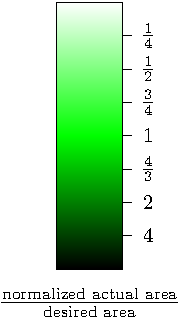
\includegraphics{Resources/Evaluation-Example-Dynamics-Legend.pdf}}
\end{tabular}
	\caption{Exemplary evolution of the generated map for an input graph with $n = 10$ at different points in time $t \in \{0,1,2,3\}$. The lightness of the region colors in the right column represents the pressure in the respective regions, with lighter regions having lower pressure than darker regions. From (a) to (b) the green-purple boundary is flipped, from (b) to (c) the red-blue boundary is flipped, and eventually from (c) to (d) the blue region is removed.}
	\label{fig:exemplary-maps-dynamics}
\end{figure}

\clearpage

\begin{figure}[H]
	\centering
	\bigdrawing{Resources/Evaluation-Example-n10-0F69CDD9-EAAD-4F81-934F-8BA98B1424F6-2.pdf}
	\bigdrawing{Resources/Evaluation-Example-n10-9A841901-DFA0-4ECD-A758-87E1C8A1D0D0-0.pdf}
	\caption{Exemplary maps produced by our framework for $n = 10$.}
	\label{fig:exemplary-maps-small}
\end{figure}

\begin{figure}[H]
	\centering
	\bigdrawing{Resources/Evaluation-Example-n20-450053F2-5F0A-4CFE-8A08-92CC201A07B9-0.pdf}
	\bigdrawing{Resources/Evaluation-Example-n20-AE097F3A-14FD-4735-A19B-8FD343CA3346-0.pdf}
	\caption{Exemplary maps produced by our framework for $n = 20$.}
	\label{fig:exemplary-maps-medium}
\end{figure}

\begin{figure}[H]
	\centering
	\bigdrawing{Resources/Evaluation-Example-n30-9BA67779-50C2-483B-8E81-916125D5D3F7-0.pdf}
	\bigdrawing{Resources/Evaluation-Example-n30-45D8EAD2-210C-4F04-8C7F-EA3E65484875-0.pdf}
	\caption{Exemplary maps produced by our framework for $n = 30$.}
	\label{fig:exemplary-maps-large}
\end{figure}
